\documentclass{article}
\usepackage{amsmath}
\usepackage{mathptmx}
\usepackage{tikz}
\usepackage{pgfplots}
\usepackage{tkz-fct}
\usetikzlibrary{angles, quotes}
\usetikzlibrary{arrows.meta, arrows}
\usepgfplotslibrary{polar}
\usepgfplotslibrary{fillbetween}
\usetikzlibrary{external}
\tikzexternalize[prefix={external/}]

\tikzset{
    export as png/.style={
        external/system call/.add={}{
            && convert -density #1 -transparent white "\image.pdf" "\image.png"
        },
    },
    export as png/.default={200},
}

\DeclareSymbolFont{symbolsb}{OMS}{cmsy}{m}{n}
\SetSymbolFont{symbolsb}{bold}{OMS}{cmsy}{b}{n}
\DeclareSymbolFontAlphabet{\mathcal}{symbolsb}
\definecolor{myblue}{rgb}{0.067,0.529,0.871}
\definecolor{mypurple}{rgb}{0.859,0.071,0.525}
\definecolor{myred}{rgb}{1.0, 0.13, 0.32}
\definecolor{mygreen}{rgb}{0.01, 0.75, 0.24}
\definecolor{myblack}{gray}{0.5}
\definecolor{mygray}{gray}{0.7}

\def\req{\protect\rotatebox{90}{$\scriptstyle=$}}

\begin{document}

\tikzset{export as png}

\tikzsetnextfilename{grafca-ext-1}
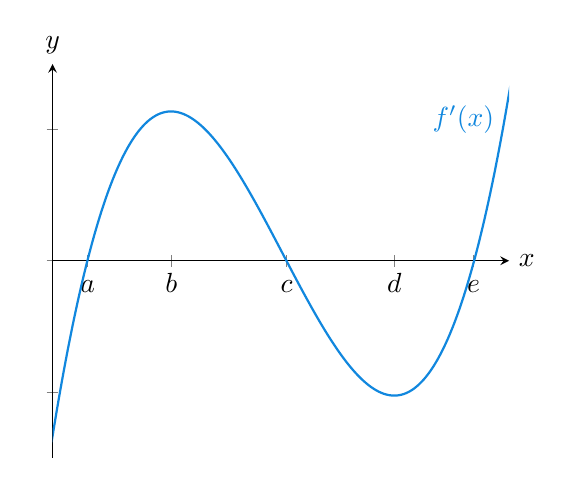
\begin{tikzpicture}[x=5cm,y=5cm]
    \begin{axis}[
    scale only axis,
    axis x line=middle,
    axis y line=left,
    xlabel={$x$},
    ylabel={$y$},
    every axis x label/.style={at={(ticklabel* cs:1)}, anchor=west,},
    every axis y label/.style={at={(ticklabel* cs:1)}, anchor=south,},
    ymin=-3, ymax=3,
    xtick={1.64, 2.41, 3.47, 4.46, 5.19},
    xticklabels={$a$, $b$, $c$, $d$, $e$},
    xticklabel style={yshift=-3ex, anchor=south},
    height=5cm,
    yticklabels={,,}
    ]
    \addplot[domain=-0.62:8.56, samples=200, smooth, myblue,thick] {1.7+3*(x-2)-4.3*(x-2)^2+(x-2)^3}
    node[left, pos=0.36] {$f'(x)$};
    \end{axis}
    \end{tikzpicture}
\end{document}


